\documentclass[../../main.tex]{subfiles}

\begin{document}

\section{Variabili cinematiche}
\begin{figure}[h!]
    \centering
    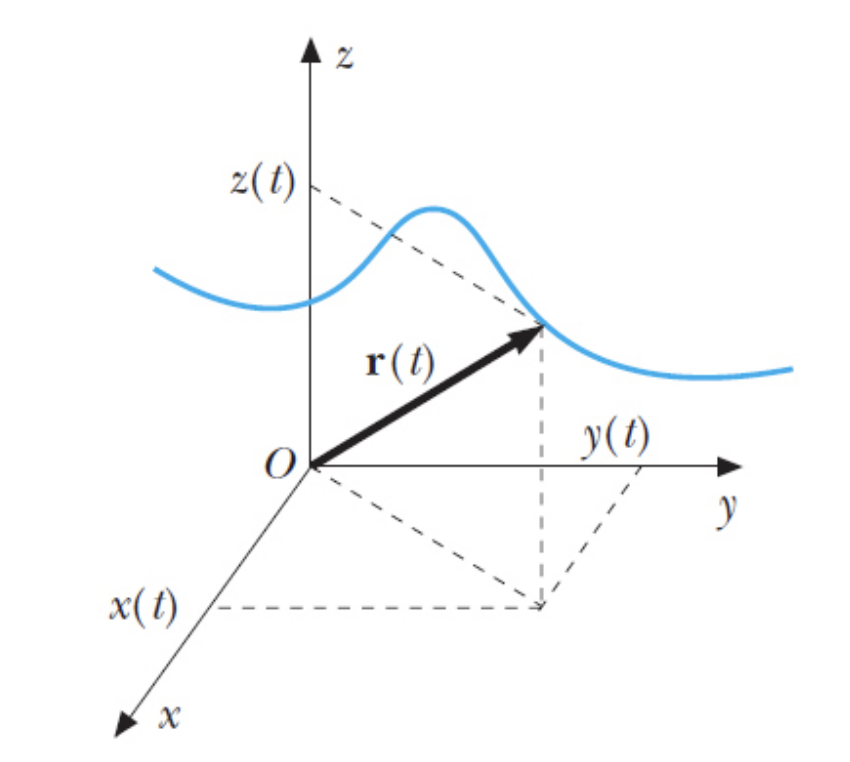
\includegraphics[width=0.5\textwidth]{traiettoria.png}
    \caption{Traiettoria di un punto}
\end{figure}
$\bar{r}(t)$ o $\overline{OP}$ vettore posizione o raggio vettore.
\[
    \bar r(t) = x(t)\bar{u}_x + y(t)\bar{u}_y + z(t)\bar{u}_z \ \ \ \textit{Legge oraria}
\]
\begin{figure}[h!]
    \centering
    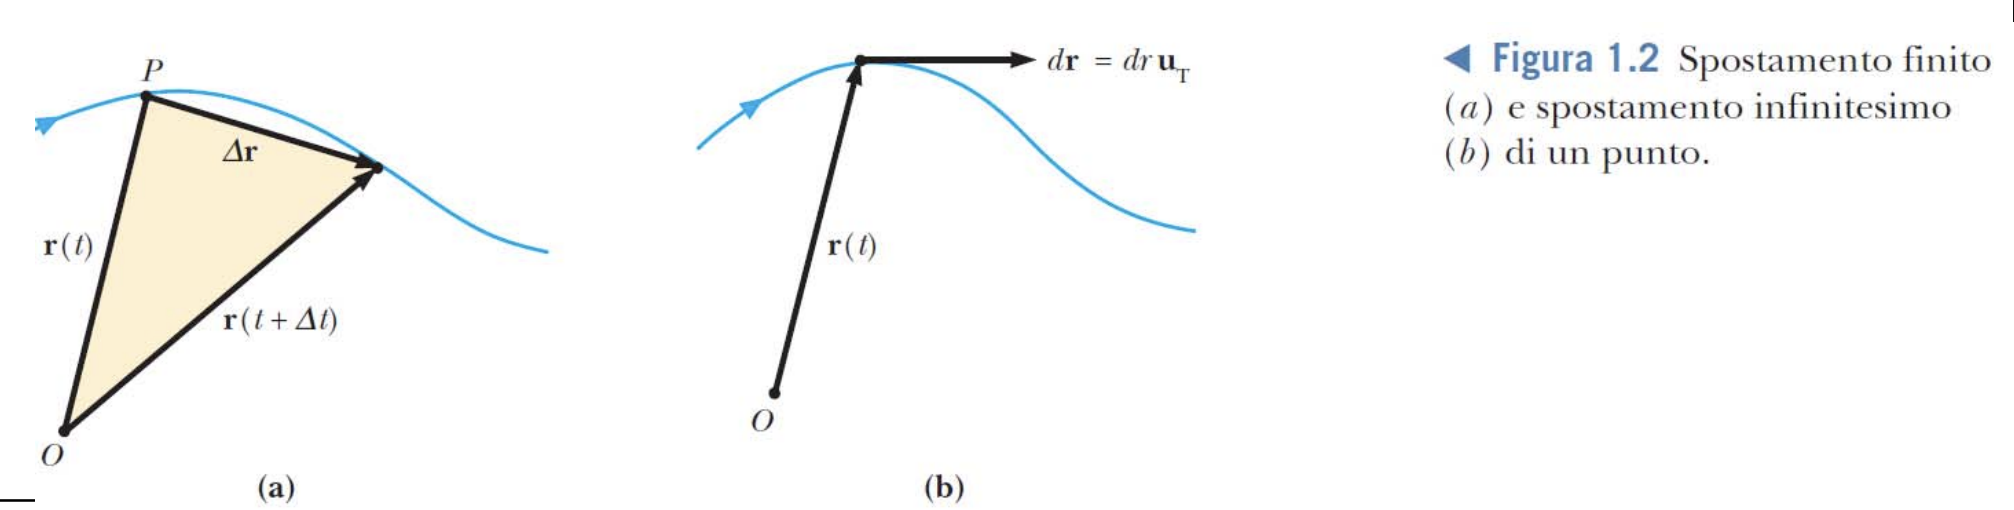
\includegraphics[width=0.5\textwidth]{velocitatangente.png}
\end{figure}
La velocità è sempre tangente alla traiettoria:
\[
    \bar{v}_m = \dfrac{\bar{r}(t + \Delta t) - \bar{r}(t)}{\Delta t} \ \ \ \textit{Velocità media}
\]
\[
    \bar{v} = \lim_{\Delta t \to 0} \dfrac{\bar{r}(t + \Delta t) - \bar{r}(t)}{\Delta t} = \dfrac{d\bar{r}}{dt} \ \ \ \textit{Derivata del vettore posizione}
\]
\[
    \bar{v} = \dfrac{dx}{dt} \bar{u}_x + \dfrac{dy}{dt} \bar{u}_y + \dfrac{dz}{dt} \bar{u}_z = v_x\bar{u}_x + v_y\bar{u}_y + v_z\bar{u}_z
\]








\end{document}